\documentclass[final]{beamer}
\usepackage[T1]{fontenc}
\usepackage[utf8]{inputenc}
\usepackage{lmodern}
\usepackage{amsmath,amssymb}
\usepackage{graphicx}
\usepackage{ragged2e}
\usepackage{array}
\usepackage{tikz}
\usepackage[size=custom,width=185,height=90,scale=1.70]{beamerposter}

\graphicspath{{./}{../figures/}}

\definecolor{FIMBlue}{RGB}{91,156,222}
\definecolor{FIMBlueDark}{RGB}{39,71,110}
\definecolor{FIMText}{RGB}{36,41,49}
\definecolor{FIMMuted}{RGB}{94,104,119}
\definecolor{FIMPanel}{RGB}{244,248,253}
\definecolor{FIMBorder}{RGB}{208,220,235}

\setbeamercolor{normal text}{fg=FIMText,bg=white}
\setbeamercolor{headline}{fg=white,bg=FIMBlueDark}
\setbeamercolor{block title}{fg=white,bg=FIMBlue}
\setbeamercolor{block body}{fg=FIMText,bg=white}
\setbeamercolor{itemize item}{fg=FIMText}
\setbeamercolor{itemize subitem}{fg=FIMText}

\setbeamerfont{title}{series=\bfseries,size=\fontsize{104}{112}}
\setbeamerfont{author}{size=\fontsize{40}{44}}
\setbeamerfont{institute}{size=\fontsize{30}{34}}
\setbeamerfont{block title}{series=\bfseries,size=\fontsize{44}{48}}
\setbeamerfont{block body}{size=\fontsize{31}{35}}
\setbeamerfont{caption}{size=\fontsize{22}{25}}

\setbeamertemplate{navigation symbols}{}
\setbeamertemplate{itemize item}{\raisebox{0.14em}{\tiny$\blacktriangleright$}}
\setbeamertemplate{itemize subitem}{\raisebox{0.14em}{\tiny$\blacktriangleright$}}
\setbeamertemplate{block begin}{%
  \vspace{0.18cm}
  \begin{center}
  \begin{beamercolorbox}[wd=0.965\linewidth,ht=1.42cm,dp=0.18cm,leftskip=0.38cm,rightskip=0.35cm]{block title}
    \usebeamerfont{block title}\strut\insertblocktitle\strut
  \end{beamercolorbox}
  \end{center}
  \vspace{0.16cm}
  \begin{beamercolorbox}[wd=\linewidth,sep=0.12cm]{block body}
    \usebeamerfont{block body}
}
\setbeamertemplate{block end}{%
  \end{beamercolorbox}
  \vspace{0.12cm}
}
\setlength{\leftmargini}{1.1em}
\setlength{\leftmarginii}{0.9em}
\setlength{\columnsep}{1.8cm}
\emergencystretch=3em

\pdfstringdefDisableCommands{%
  \def\textsuperscript#1{ (#1)}%
  \def\and{, }%
}

\hypersetup{
  pdftitle={In-Context Learning of Temporal Point Processes with Foundation Inference Models},
  pdfauthor={David Berghaus, Patrick Seifner, Kostadin Cvejoski, Cesar Ojeda, Ramses J. Sanchez}
}

\title{In-Context Learning of Temporal Point Processes\\with Foundation Inference Models}
\author{David Berghaus\textsuperscript{1,2} \and Patrick Seifner\textsuperscript{1,3} \and Kostadin Cvejoski\textsuperscript{4} \and C\'esar Ojeda\textsuperscript{5} \and Rams\'es J. S\'anchez\textsuperscript{1,2,3}}
\institute{\textsuperscript{1}Lamarr Institute \quad \textsuperscript{2}Fraunhofer IAIS \quad \textsuperscript{3}University of Bonn \quad \textsuperscript{4}JetBrains Research \quad \textsuperscript{5}University of Potsdam}

\newcommand{\FIM}{\textbf{FIM-PP}}
\newcommand{\FIMzs}{\textbf{FIM-PP} (zero-shot)}
\newcommand{\FIMft}{\textbf{FIM-PP} (fine-tuned)}
\newcommand{\dataset}[1]{\textbf{#1}}

\newcommand{\subhead}[1]{\vspace{0.25em}{\color{FIMText}\bfseries #1}\par\vspace{0.2em}}
\newcommand{\emline}[1]{{\color{FIMBlueDark}\bfseries #1}}
\newcommand{\logoimg}[1]{\includegraphics[height=6.1cm,keepaspectratio]{#1}}
\newcommand{\tightfigure}[3]{%
  \begin{figure}
    \centering
    \includegraphics[width=\linewidth,height=#2,keepaspectratio]{#1}
    \caption{#3}
  \end{figure}
}
\newcommand{\eqpanel}[1]{%
  \begin{beamercolorbox}[wd=\linewidth,rounded=true,sep=0.7em]{block body}
    #1
  \end{beamercolorbox}
}
\newcommand{\metricbox}[2]{%
  \begin{beamercolorbox}[wd=\linewidth,rounded=true,sep=0.85em]{block body}
    {\color{FIMBlueDark}\bfseries #1}\par
    \vspace{0.2em}
    #2
  \end{beamercolorbox}
}

\begin{document}
\begin{frame}[t]

\begin{beamercolorbox}[wd=\paperwidth,sep=1.35cm,leftskip=3.8cm,rightskip=2.0cm]{block body}
  \begin{columns}[T,totalwidth=\textwidth]
    \begin{column}{0.59\textwidth}
      \hspace*{0.9cm}\parbox[t]{0.94\linewidth}{%
        {\usebeamerfont{title}\color{FIMText}\inserttitle\par}
        \vspace{0.6cm}
        {\usebeamerfont{author}\color{FIMText}\insertauthor\par}
        \vspace{0.25cm}
        {\usebeamerfont{institute}\color{FIMMuted}\insertinstitute\par}
        \vspace{0.25cm}
        {\usebeamerfont{institute}\color{FIMMuted}\textit{Contact:} david.berghaus@iais.fraunhofer.de \quad \textit{Project:} fim4science.github.io/OpenFIM/intro.html\hspace{0.55cm}\raisebox{-0.6cm}{
\includegraphics[height=2.7cm]{qrcode.svg.png}}}
      }
    \end{column}
    \begin{column}{0.41\textwidth}
      \centering
      \makebox[\linewidth][c]{%
        \logoimg{lamarr-logo-2023.png}%
        \hspace{2.8cm}%
        \logoimg{uni_bonn.png}%
        \hspace{2.8cm}%
        \logoimg{iais.png}%
        \hspace{2.8cm}%
        \logoimg{tu-potsdam.pdf}%
      }
    \end{column}
  \end{columns}
\end{beamercolorbox}

\vspace{0.35cm}

\begin{columns}[T,totalwidth=\textwidth]
  \begin{column}{0.285\textwidth}

    \begin{block}{Summary}
      \justifying
      Modeling irregular marked event sequences as temporal point processes gives an interpretable description of \emph{when} events occur and \emph{which type} they have. Existing neural TPP models usually learn \emph{one dataset at a time}. \FIM is a pretrained recognition model that infers conditional intensities \emph{in context} from a set of related event sequences.

      \vspace{0.35em}
      We pretrain on \emline{72K synthetic processes / 14.4M events}. The same model can then be applied \emline{zero-shot} to real-world event data or adapted within minutes by \emline{fine-tuning}.

      \vspace{0.6em}
      \metricbox{Key message}{One pretrained model already competes with specialized TPP baselines; fine-tuning turns that prior into the strongest long-horizon performer.}
    \end{block}

    \begin{block}{Motivation and Goals}
      \subhead{Marked temporal point processes}
      \noindent
      \begin{minipage}[t]{0.58\linewidth}
      \vspace{0pt}%
        A marked temporal point process describes an event history
        $\mathcal{H}_t=\{(t_1,k_1),\dots,(t_n,k_n)\}$ through a conditional intensity
        $\lambda(t,k \mid \mathcal{H}_t)$ that determines how likely an event of mark $k$
        is to occur at time $t$ given the past.

        \vspace{0.25em}
        \subhead{What we want}
        From a \emph{set of observed sequences} from one system, infer an interpretable
        mark-wise intensity model that transfers across datasets without retraining from scratch each time.

        \vspace{0.15em}
        \subhead{Why current practice is limiting}
        {\setlength{\itemsep}{0.1em}
        \begin{itemize}
          \item Standard neural TPPs relearn for every dataset.
          \item Zero-shot application is largely unavailable.
        \end{itemize}}

        \vspace{0.1em}
        \subhead{What \FIM changes}
        {\setlength{\itemsep}{0.1em}
        \begin{itemize}
          \item Pretrain once on a broad synthetic prior.
          \item Infer new dynamics directly from context.
          \item Keep access to an explicit intensity estimate.
        \end{itemize}}%
      \end{minipage}\hspace{0.03\linewidth}%
      \begin{minipage}[t]{0.34\linewidth}
      \vspace{0pt}%
        \centering
        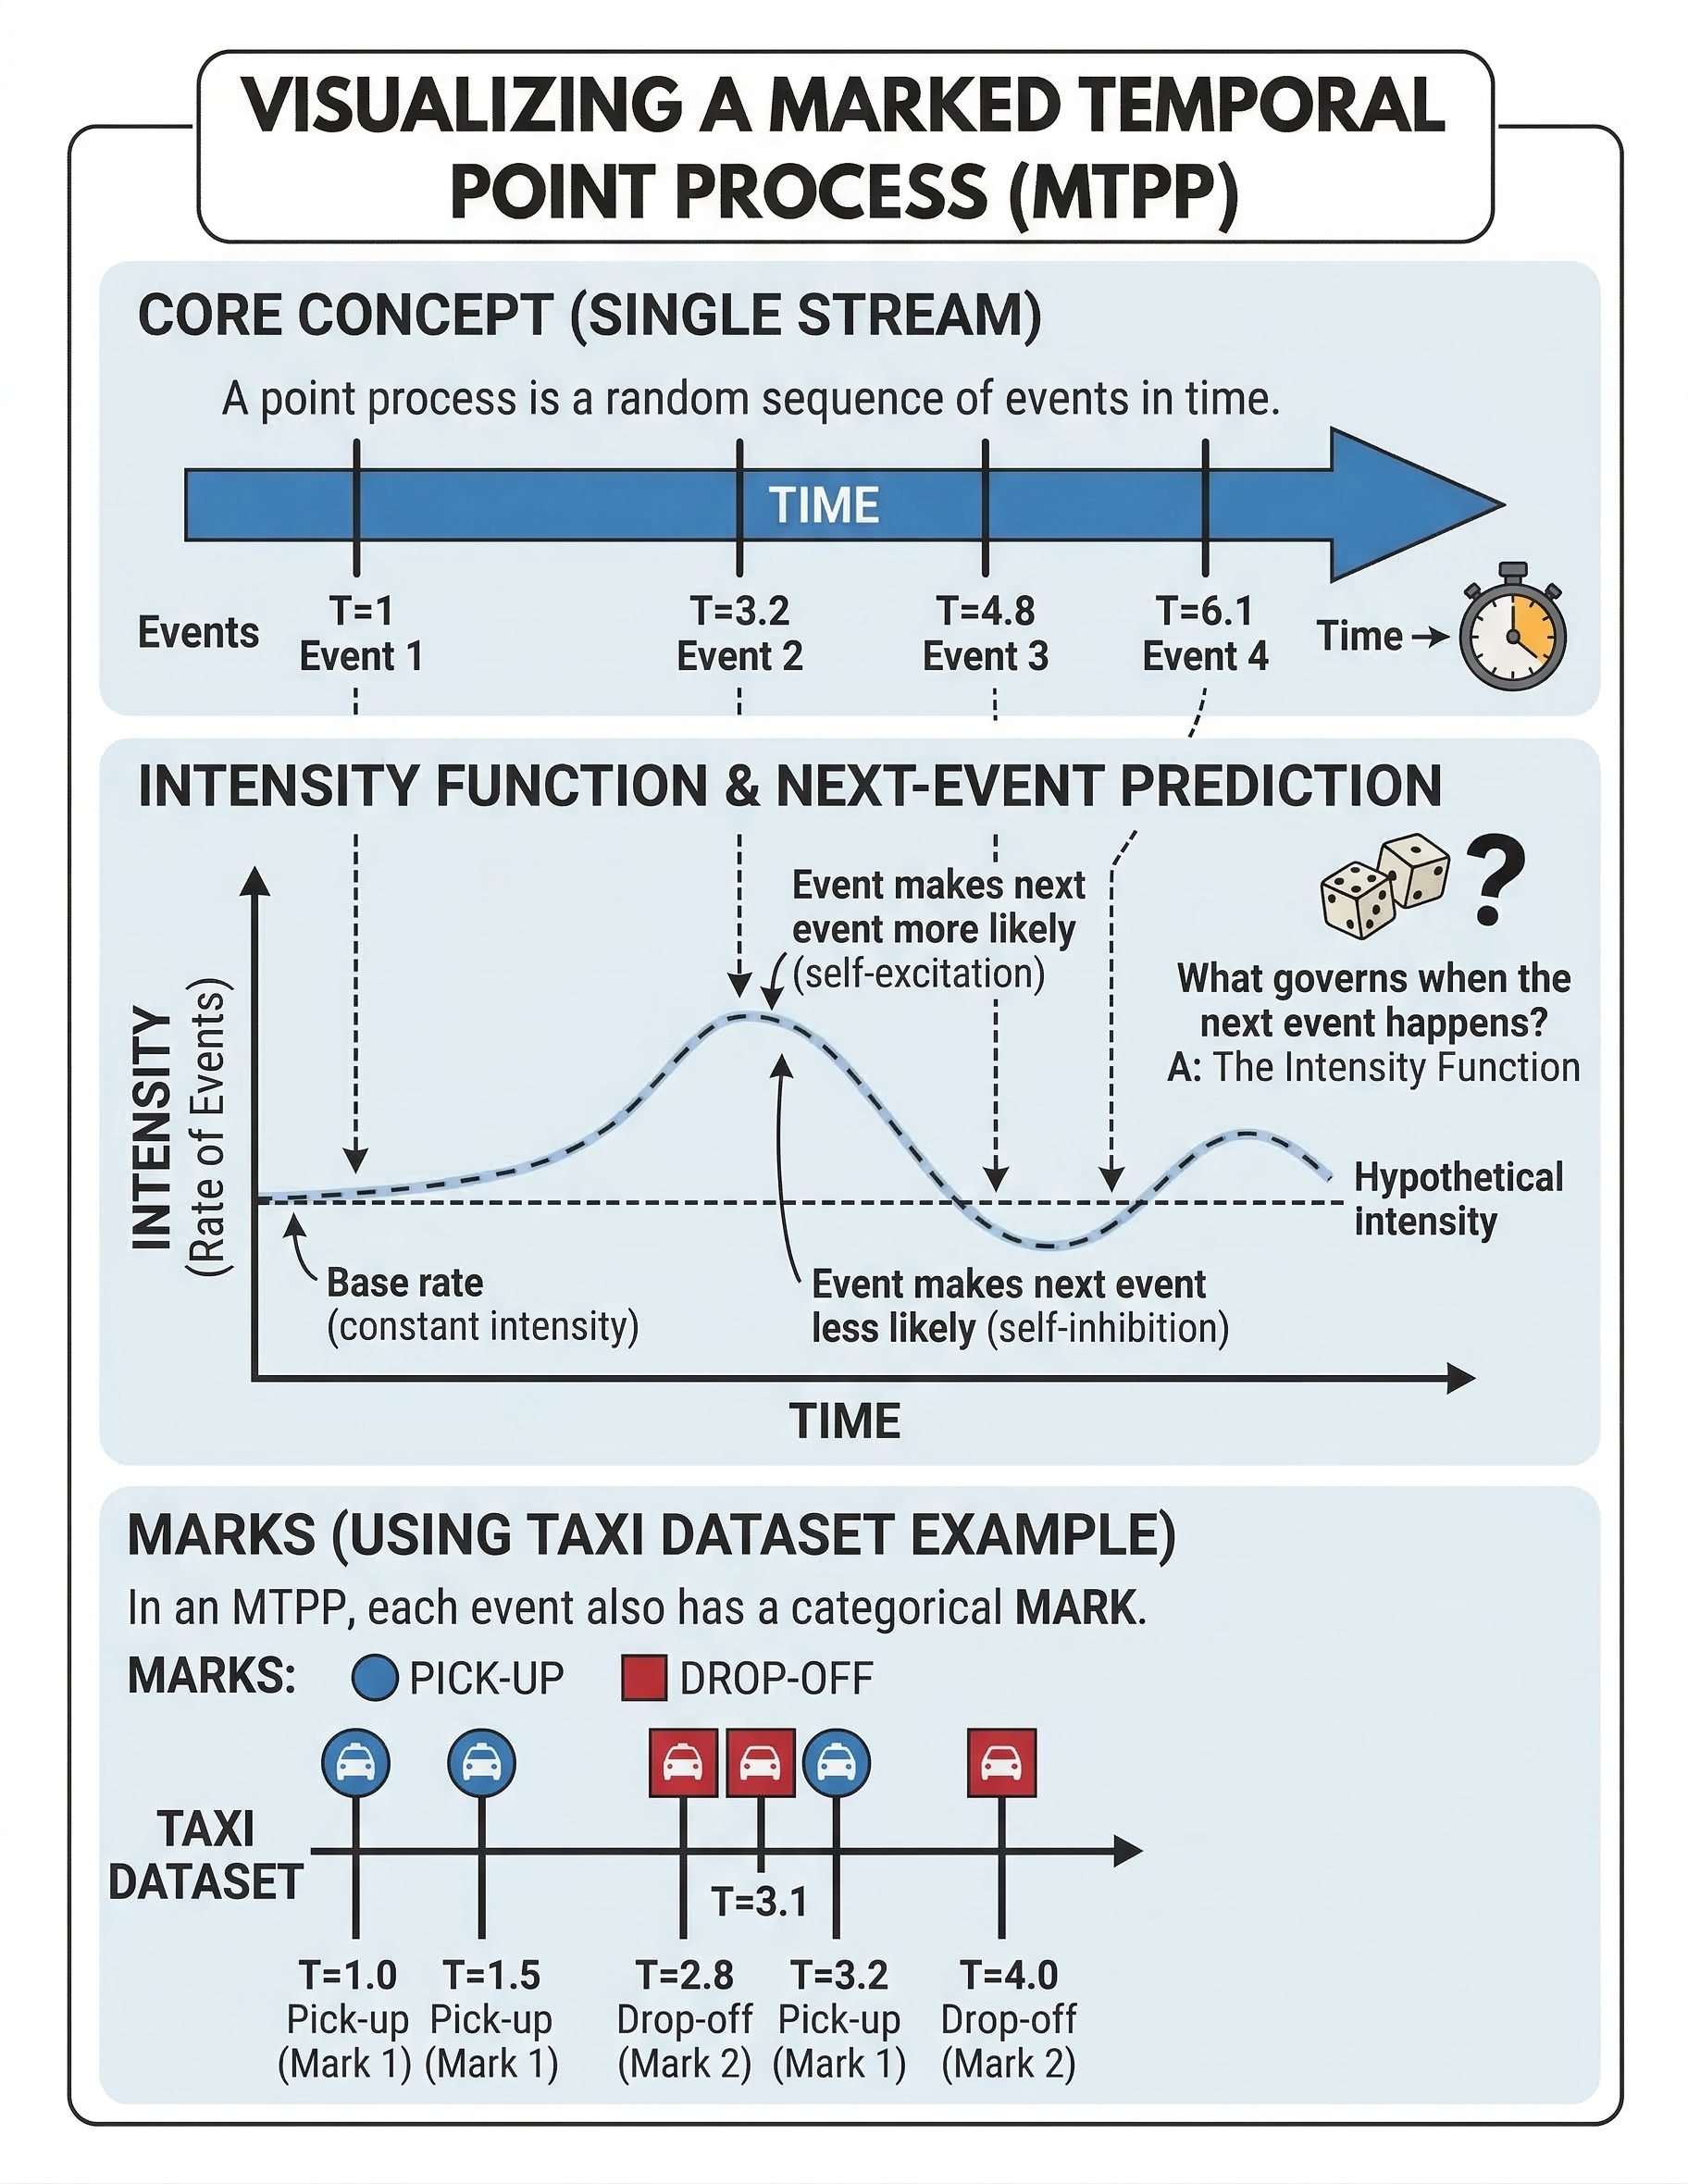
\includegraphics[width=\linewidth,height=28cm,keepaspectratio]{pp_visualization.jpeg}%
      \end{minipage}
    \end{block}

  \end{column}

  \begin{column}{0.325\textwidth}

    \begin{block}{Foundation Inference Models}
      \subhead{Part A: Synthetic training data generation}
      We sample processes from a broad prior over conditional intensities
      \[
      \lambda(t,k \mid \mathcal{H}_t)=
      \max\!\left(0,\mu_k(t)+\sum_{(t',k')\in\mathcal{H}_t} z_{kk'}\,\gamma_{kk'}(t-t')\right),
      \]
      where $\mu_k(t)$ is chosen as either a \emline{constant}, a \emline{positive sinusoid}, or a \emline{Gamma-shaped initial-rate function}, and $\gamma_{kk'}(t)$ is chosen as either \emline{zero}, an \emline{exponential Hawkes kernel}, or a \emline{shifted Rayleigh kernel}. Interaction signs $z_{kk'} \in \{-1,0,1\}$ cover \emph{excitatory}, \emph{inhibitory}, and \emph{neutral} relations.

      \vspace{0.35em}
      \subhead{Part B: Amortized inference model}
      \begin{figure}
        \centering
        
\includegraphics[width=\linewidth,height=24cm,keepaspectratio]{fim_pp_architecture_figure.pdf}
      \end{figure}
      {\itshape Context is encoded first, target-history queries then attend to it, and a mark-conditioned head predicts intensity parameters.\par}

      \vspace{0.2em}
      \begin{itemize}
        \item Context sequences are embedded from event times, marks, and inter-event times.
        \item The target history queries the learned context representation.
        \item The final mark-conditioned output predicts an interpretable intensity function.
      \end{itemize}

      \vspace{0.2em}
      \subhead{Part C: Intensity head}
      The model outputs a mark-wise conditional intensity, which can directly show self-excitation, inhibition, and time-varying event likelihood.

      \vspace{0.2em}
      \tightfigure{intensity_comparison_synth_vs_retweet.pdf}{16cm}{The pretrained model matches synthetic Hawkes intensities and also recovers meaningful excitation/inhibition structure on \dataset{Retweet}.}

      \vspace{0.25em}
      \subhead{Part D: Training and fine-tuning}
      Pretraining uses synthetic sequences and next-event likelihood. At application time, the model is used directly in \FIMzs mode or adapted on the target dataset in \FIMft mode, which typically takes only a few minutes and less than 11 GB of GPU memory.
    \end{block}

  \end{column}

  \begin{column}{0.345\textwidth}

    \begin{block}{Long-Horizon Prediction: $N=20$}
      {\fontsize{20}{24}\selectfont
      \centering
      \renewcommand{\arraystretch}{1.18}
      \setlength{\tabcolsep}{7pt}
      \resizebox{\linewidth}{!}{%
      \begin{tabular}{lcccccccc}
      & \multicolumn{2}{c}{\textbf{Taxi}} & \multicolumn{2}{c}{\textbf{StackOverflow}} & \multicolumn{2}{c}{\textbf{Amazon}} & \multicolumn{2}{c}{\textbf{Retweet}} \\
      \cline{2-3}\cline{4-5}\cline{6-7}\cline{8-9}
      Method & OTD & sMAPE & OTD & sMAPE & OTD & sMAPE & OTD & sMAPE \\
      \hline
      HYPRO & 21.60 & 93.8 & 42.40 & 111.0 & 38.6 & 82.5 & 61.03 & 106.11 \\
      Dual-TPP & 24.48 & 95.2 & 41.75 & 117.58 & 42.6 & 86.5 & 61.10 & 106.90 \\
      A-NHP & 24.76 & 97.4 & 42.59 & 108.54 & 39.5 & 84.3 & 60.63 & 107.23 \\
      NHP & 25.11 & 96.5 & 43.79 & 116.95 & 42.6 & 92.1 & 60.95 & 107.08 \\
      IFTPP & 24.05 & 95.7 & 46.28 & 115.12 & 43.8 & 90.9 & 61.72 & 106.71 \\
      TCDDM & 22.15 & 90.6 & 42.13 & 107.66 & 42.2 & 83.8 & 60.50 & 106.05 \\
      CDiff & 21.01 & 88.0 & 41.25 & 106.18 & 37.7 & 82.0 & 60.66 & 106.18 \\
      \hline
      \FIMzs & 23.15 & \textbf{76.8} & 49.26 & 96.36 & 46.2 & 128.6 & 60.24 & 99.07 \\
      \FIMft & \textbf{17.91} & 76.8 & \textbf{39.80} & \textbf{88.25} & \textbf{37.2} & \textbf{81.2} & \textbf{59.44} & \textbf{87.59} \\
      \end{tabular}
      }
      \par}
    \end{block}

    \begin{block}{Next-Event Prediction}
      {\fontsize{22}{26}\selectfont
      \centering
      \renewcommand{\arraystretch}{1.18}
      \setlength{\tabcolsep}{8pt}
      \resizebox{0.98\linewidth}{!}{%
      \begin{tabular}{lccc|ccc}
      & \multicolumn{3}{c|}{\textbf{Taxi}} & \multicolumn{3}{c}{\textbf{Taobao}} \\
      \cline{2-7}
      Method & RMSE$_{\Delta t}$ & Acc & sMAPE$_{\Delta t}$ & RMSE$_{\Delta t}$ & Acc & sMAPE$_{\Delta t}$ \\
      \hline
      A-NHP & \textbf{0.32} & \textbf{0.91} & \textbf{85.13} & 0.53 & 0.47 & 129.13 \\
      Dual-TPP & 0.34 & \textbf{0.91} & 89.12 & 0.53 & 0.47 & 131.43 \\
      NHP & 0.34 & \textbf{0.91} & 90.63 & 0.53 & 0.46 & 133.69 \\
      IFTPP & 0.38 & 0.90 & 90.03 & 0.53 & 0.45 & 126.01 \\
      CDiff & 0.34 & \textbf{0.91} & 87.12 & 0.52 & 0.48 & 127.12 \\
      \hline
      \FIMzs & 0.34 & 0.47 & 98.03 & \textbf{0.13} & 0.52 & \textbf{112.89} \\
      \FIMft & 0.45 & \textbf{0.91} & 85.91 & 0.16 & \textbf{0.60} & 115.98 \\
      \end{tabular}
      }
      \par}
    \end{block}

  \end{column}
\end{columns}

\end{frame}
\end{document}
